\documentclass[a4paper, 11pt]{article} 

\usepackage{fullpage}
\usepackage{amssymb}
\usepackage{amsmath}

\usepackage{tikz-qtree}
\usepackage{tikz}
\usetikzlibrary{calc,fit,trees}

\title {Logic Programming - Resolution}

\begin{document}
	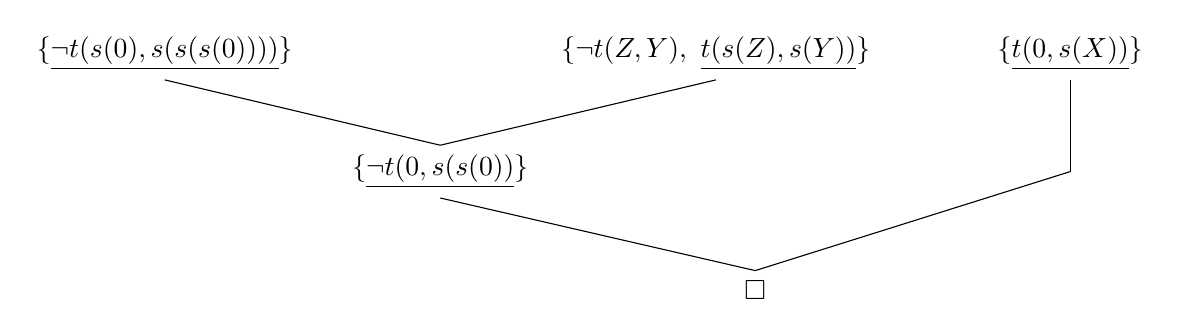
\begin{tikzpicture}[
		grow'=up,
		level 1/.style={sibling distance=80mm},
		level 2/.style={sibling distance=70mm},
		level 3/.style={sibling distance=50mm}
	]
	\node {$\square$} 
		child {node{$\{\underline{\neg t(0,s(s(0))}\}$}
			child {node{$\{\underline{\neg t(s(0),s(s(s(0))))}\}$}}
			child {node{$\{\neg t(Z,Y),\ \underline{ t(s(Z),s(Y))}\}$}}
		}
      		child { 
      			child {node  {$\{\underline{t(0,s(X))}\}$}}
      		};
      \end{tikzpicture}
\end{document}
